\section{Normalisation method}
\label{sec:Normalisation}
The branching fraction of a \Bmumumu signal is obtained by normalising to the \bjpsimumuk decay as
\begin{equation}
  \begin{aligned}
    \label{eq:BF}
	\mathcal{B}(\Bmumumu) &=\mathcal{B}(\decay{\Bp}{\jpsi\Kp}) \times
	\mathcal{B}(\decay{\jpsi}{\mup\mun}) \\
	 &\phantom{{}={}} \times
	\frac{\varepsilon(\decay{\Bp}{\jpsi\Kp})}{\varepsilon(\Bmumumu)}
	\times \frac{N(\Bmumumu)}{N(\decay{\Bp}{\jpsi\Kp})},
\end{aligned}
\end{equation}
where $N$ is the yield of the decay, $\varepsilon$ is the overall efficiency
to reconstruct and select the decay. The braching fractions are taken from
Ref.~\cite{PDG2018}.

The \decay{\Bp}{\jpsi\Kp} candidates are selected in the same way as the signal, except that
the third particle must be consistent with the kaon hypothesis and the dimuon mass
consistent with the $\jpsi$ mass. This reduces the
impact of systematic uncertainties related to the ratio of efficiencies in
Eq.~(\ref{eq:BF}). Most of the signal and normalisation selection efficiencies are
estimated using simulation. Efficiencies of the PID are obtained using control data
samples where identities of the final-state particles can be deduced from the kinematics
of the decay. The total efficiency of the \Bmumumu signal is around $37\%$ relative
to the normalisation channel. This lower efficiency is caused by the lower dimuon
mass for the signal that affects the trigger, reconstruction and BDT efficiencies.
The muon PID requirements are also less efficient due to the sharing of muon hits
between the different final-state muons in the signal decay.

\begin{figure}[t]
\centering
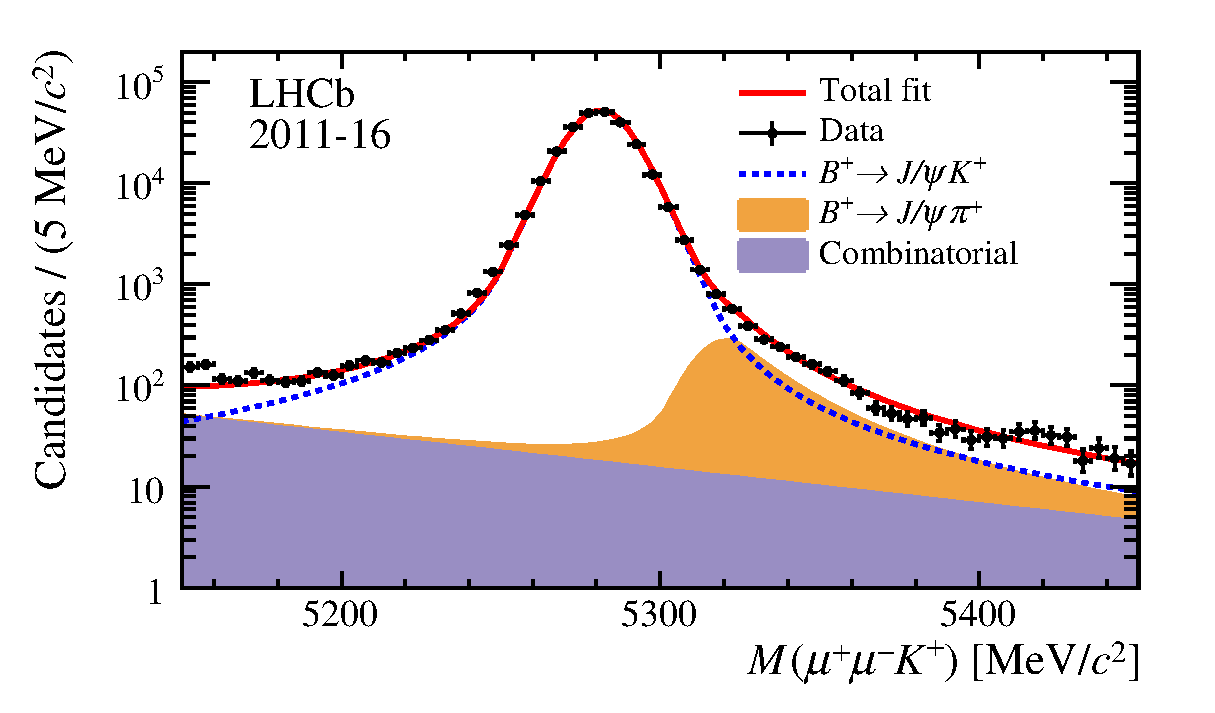
\includegraphics[width=0.85\linewidth]{Figure_2.eps}
\caption{\small Fit to the mass distribution of the selected $\decay{\Bp}{\jpsi\Kp}$ candidates. The combinatorial background (purple) and misidentified \decay{\Bp}{\jpsi\pip} decays (orange) are stacked up while the $\decay{\Bp}{\jpsi\Kp}$ signal is shown as a dashed line. The data points are shown as black points with the total fit overlaid as a red solid line.}
\label{fig:cfit}
\end{figure}
The \decay{\Bp}{\jpsi\Kp} yield is determined by performing an unbinned extended
maximum-likelihood fit to the $\mu^{+} \mu^{-} K^{+}$ mass distribution.
The shape of the \mbox{\decay{\Bp}{\jpsi\Kp}} mass distribution is described by a
Hypatia function~\cite{Santos:2013gra} that accounts for non-Gaussian tails on both
sides of the peak. In the fit, the mean and width parameters are allowed
to vary and all other parameters are determined from simulation. The 
shape of the misidentified background contribution of \decay{\Bp}{\jpsi\pip} 
decays is modelled with a Gaussian core with power law tails on each 
side of the peak. The mean and width are allowed to vary freely in 
the fit while the tail parameters are determined from simulation.
Combinatorial background is parameterised with an exponential function
with a decay constant that is allowed to vary in the fit. The result of
the fit is shown in Fig.~\ref{fig:cfit} and yields $2.7\times 10^5$
\decay{\Bp}{\jpsi\Kp} decays.

